\documentclass{minimal}
\usepackage{tikz}
\usetikzlibrary{arrows,positioning} 
\tikzset{
    %Define standard arrow tip
    >=stealth',
    %Define style for boxes
    punkt/.style={
           rectangle,
           draw=black, very thick,
           text width=10.5em,
           minimum height=2em,
           text centered},
    % Define arrow style
    pil/.style={
           ->,
           thick,
           shorten <=2pt,
           shorten >=2pt,}
}
\begin{document}

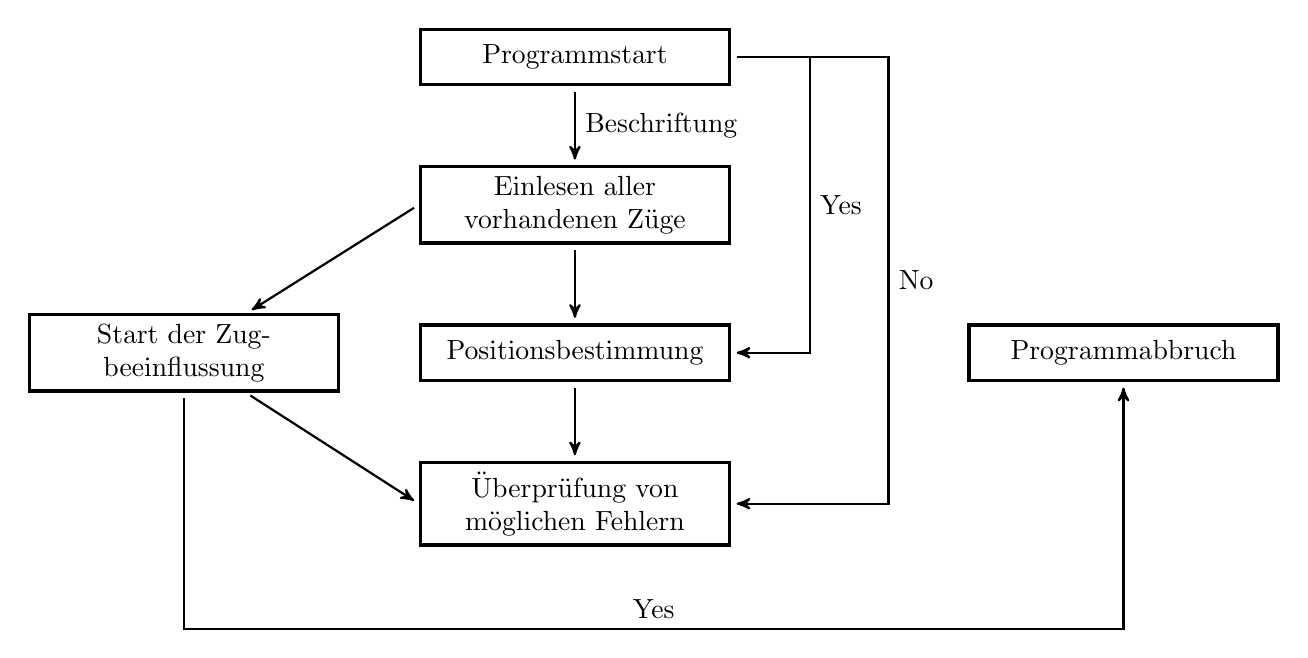
\begin{tikzpicture}[node distance=1cm, auto,]




%nodes
\node[punkt] (a) {Programmstart};
\node[below=of a, punkt] (b) {Einlesen aller vorhandenen Züge};
\node[below=of b, punkt](c) {Positionsbestimmung};
\node[below=of c, punkt] (d) {Überprüfung von möglichen Fehlern};
\node[left=of c, punkt] (e) {Start der Zugbeeinflussung};
\node[right= 3cm of c, punkt] (f) {Programmabbruch};
 
\draw [pil] (a) -- node[pos=0.5] {Beschriftung} (b);
\draw [pil] (b) -- (c);
\draw [pil] (c) -- (d);
\draw [pil] (b.west) -- (e);
\draw [pil] (e) -- (d.west);

\draw [pil] 
    (a.east) -- +(2,0) |- node[pos=0.25] {No} (d.east);
    
\draw [pil] 
    (a.east) -- +(1,0) |- node[pos=0.25] {Yes} (c.east); 
    
\draw [pil] 
    (e.south) -- +(0,-3) -| node[pos=0.25] {Yes} (f.south); 


 

 

\end{tikzpicture}
\end{document}

